%\documentclass[aps,prl,preprint,groupedaddress]{revtex4-1}
%\documentclass[aps,prl,preprint,superscriptaddress]{revtex4-1}
\documentclass[aps,prl,twocolumn,superscriptaddress]{revtex4-1}
%\documentclass[aps,pre,preprint,superscriptaddress]{revtex4-1}
%\documentclass[aps,pre,preprint,groupedaddress{revtex4-1}
\usepackage{graphicx}% Include figure files
\usepackage{dcolumn}% Align table columns on decimal point
\usepackage{bm}% bold math
\usepackage[centertags]{amsmath}
\usepackage{amsfonts}
\usepackage{amssymb}
\usepackage{amsthm}
\usepackage{newlfont}
\usepackage{color}
\usepackage{natbib}
\usepackage{subfigure}

 
\begin{document}

\title{Fast and Accurate Determination of Phase Transition Temperature in Computer Simulation}

\author{Mingzhe Shao}
\affiliation{Department of Packaging and Printing, Tianjin University of Science and Technology, Tianjin, China}

\author{Xin Zhou$^{*}$}
\affiliation{School of Physical Sciences, University of Chinese Academy of Sciences, Beijing 100049 China}

\date{\today}
 

\begin{abstract}  
Generalized canonical ensemble (GCE) simulations are performed in water/ice coexisting systems to obtain its phase transition temperature. For the first time, the equilibrium at water/ice coexisting state can be studied in an individual simulation. This equilibrium, no longer a stochastic process, leads to a remarkable increase in both efficiency and accuracy of determining melting points. In this study, TIP4P/2005, TIP4P/ICE, mW water model are applied to build Ice Ih/water two-phase systems, then equilibrated at distinct areas in energy surface. States such as bulk water, ice and water/ice coexisting have been evolved, and their corresponding temperature are gained at the same time. The result of phase transition temperature is in excellent agreement with previous studies, is 253K, 272K, and 274K, respectively. Results from small systems show subtle accuracy lost.  These features make GCE approach determining phase transition temperature robust, easy to use, and particularly good at working on computationally expensive systems.
\end{abstract}

\pacs{ } 

\maketitle{}
\section{Introduction}

The transition between different molecular structures induce significant changes in physical properties.  However, these changes are not yet well understood in many transitions, their mechanism at the molecular level remains largely unknown.
exp1:The transition between the ferromagnetic and paramagnetic phases of magnetic materials at the Curie point.
exp2:transition into superconductive state.
exp3: Hydrogen bonding between individual water molecules yields a disordered three-dimensional hydrogen-bond network whose rugged and complex global potential energy surface permits a large number of possible network configurations, ~\cite{Matsumoto2002} making water freezing one of the most intriguing phase transition system. 
These issues call forth more comprehensive knowledge of phase transition, especially the details in phases-coexisting systems(PCS). Studying PCS by performing direct canonical or isothermal–isobaric(NPT) ensemble is well performed worldwide and generally accepted, however the efficiency of this approach is largely determined by the nucleation energy barrier of PCS. Sampling critical states is hard since surface tension increased system energy leads to a less probability of being occupied. Besides, studying thermodynamics by sampling in non-equilibrium systems is controversial. 

Estimating transitional temperature is of absolute importance in describing PCS. The technique of direct coexistence is a first choice, studies have been carried out by simulating PCS in a temperature range, order parameters such as density are used to monitor the transition process. Transitional temperature is thus determined as the spinodal temperature of order parameter. However, evolution of states at critical temperature is stochastic, accuracy of this approach depends on not only sensitiveness of order parameter and the temperature interval in simulations, the sample volume matters as well. Another method is proposed by fitting the temperature dependence of free energy for both two phase, the intersection stands for the transitional temperature. This method shows better precision, but estimating free energy of systems is not convenient and takes extra work.

In this work, we aim to provide a simple method of high-precision and efficiency for determining the phase transition temperature in PCS. To achieve such goal, generalized canonical ensemble (GCE) has been implemented successfully in ice Ih/water PCS with mW, TIP4P-2005 and TIP4P-ICE water models. GCE can sufficiently visit the phase-coexistence regions and its energy distribution can be Gaussian-like. Thus the stochastic nature of phase transition can be largely get rid of, making one single simulation enough to estimate phase transition temperature. Besides the enhanced sampling in GCE expanded sample volume insure considerable precision of estimation.

This work is organized as follows: Sec. II describes the models and methodology used in this work. Section III presents the results for phase-coexistence region for different water potential models. The papers ends with a final discussion and the conclusions of this work.
\section{Models and Methods} 
\subsection{A. Water Models}
So far, water has been modeled in several different manner such as multi-site model\cite{Sanz2004,Bryk2002,Horn2005,Gonzalez2010,Kumar2012,Sedlmeier2011,Vega2007,Yu2013,Himoto2011}, implicit model\cite{Huißmann2012}, coarse-grained model\cite{Molinero2009,Marrink2004Coarse}. Multi-site mode have been widely applied to reveal the thermodynamic, dynamic, and structural anomalies of water\cite{Gao2000,Bryk2002,Sanz2004}, but some times computations can be very time-consuming, especially when it comes to water freezing at low supersaturation\cite{Mishima1998} . To observe puzzling behavior of water close and inside "no man's land"\cite{Moore2011}, a coarse-grained model mW water\cite{Molinero2009} using Stillinger-Weber (SW) potential to describe the tetrahedral hydrogen bond network in water and ice has been developed to accelerate the computation. In this paper, tip4p-2005, tip4p-ice and mW water models were applied to verify our method in determining phase transition temperature. In Table\ref{table:water model}  we present the parameters of water models used in this work. 

\subsection{B. GCE/GNPT Method}

Generalized canonical ensemble(GCE)\cite{Xu2012} was first proposed to enhance sampling in systems with complex energy landscape. It is a direct generalization of canonical ensemble and can be regarded as a derivative of Hetherington's Gaussian ensemble.The conformational distribution $W_{gce}$ for GCE ensemble $f_{gce}{E}$ is

\begin{equation}
W_{gce}=exp[−f_{gce}(E)]\;,
\end{equation}

while $f_{gce}(E)$ is a particular function, or say, effective potential function in GCE, defined as
\begin{equation}
f_{gce}(E)=\beta E+ \frac{\alpha}{2}(E−U)^2\;.
\end{equation}
$\beta$, $\alpha$ and U are three parameters adjustable to control the energy distribution of system. It is an usual canonical ensemble if $\alpha=0$. The GCE ensemble can easily be obtained by setting the instant thermal coupling temperature as the first order derivative of ensemble function:
\begin{equation}
\widetilde{\beta}(E)≡\frac{f_{gce}(E)}{dE}≡\beta+α(E−U)\;,
\end{equation}
To expand the universality of this method, a generalized isobaric-isothermal ensemble(GNPT) was developed in the same way, by defining ensemble function of entropy $H=E+PV$ rather than $E$:

\begin{equation}
f_{gce}(H)=\beta H+ \frac{\alpha}{2}(H−U)^2\;.
\end{equation}
and corresponding instant thermal coupling temperature as
\begin{equation}
\widetilde{\beta}(H)≡\frac{f_{gnpt}(H)}{dH}≡\beta+α(H−U)\;,
\end{equation}

In a word,  GCE/GNPT can be applied to sufficiently visit the phase-coexistence regions, its energy distribution is Gaussian-like\cite{Xu2012,Xu2015}. And for the first time, this method is used to determine the phase transition temperature.

\subsection{C. Simulation Details}
In our work, system is built with 32480 or 4584 water molecules for mW (approximately 400 Å × 56 Å × 43 Å) and full atom water model (approximately 200 Å × 26 Å × 29 Å), respectively. Ice phase is extract from 20ns equilibrated bulk ice Ih at 260K, with x-y plane set as ice Ih basal plane, leaving the secondary prismatic plane ($1\overline{2}10$) in contact with bulk water. The two phases system are equilibrated for another 100 ps to produce the interfaces. The size in x direction is about 7 time of y and z direction, to ensure stable interfaces and study size effect in measuring phase transition temperature. Besides, systems of distinct size have been carried out to test the universality of this method.

All MD simulations were carried out in GNPT employing LAMMPS molecular dynamics code with GCE module\cite{Xu2012}. A Nosé−Hoover thermostat and barostat\cite{Nose1984,Hoover1985} with  relaxation times 0.1 and 1 ps are used to keep the temperature and pressure fixed. For full atom water model, a time step of 2\,fs  was used in all simulations. Lennard-Jones interactions are truncated smoothly at 14.0 Å. Nontruncated electrostatic interactions are treated by the particle-particle particle mesh solver (pppm) with a real space cutoff of 11.0 Å and precision tolerance of $10^{-5}$.  The mW water is built by following previous work of Molinero and co-workers\cite{Molinero2009} .
\section{Results and Discussion} 

Fig.\ref{fig:conformation}
\begin{figure}[ht]
\centering{}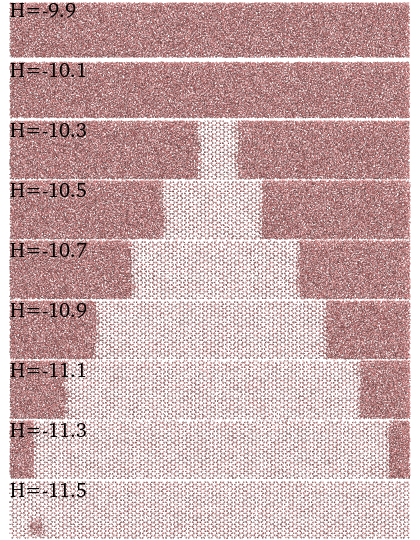
\includegraphics[width=0.5\textwidth]{conf.png} 
\caption{The conformation of GNPT ensemble at distinct energy levels: From bulk water above room temperature to completely freezed ice Ih.
\label{fig:conformation} }
\end{figure}

as Fig.\ref{fig:evolution}
the ensembles attained equilibrium in 2ns, 20ns equilibrium has been performed, data sample from 5ns to 20ns are used. 
\begin{figure}[ht]
\centering{}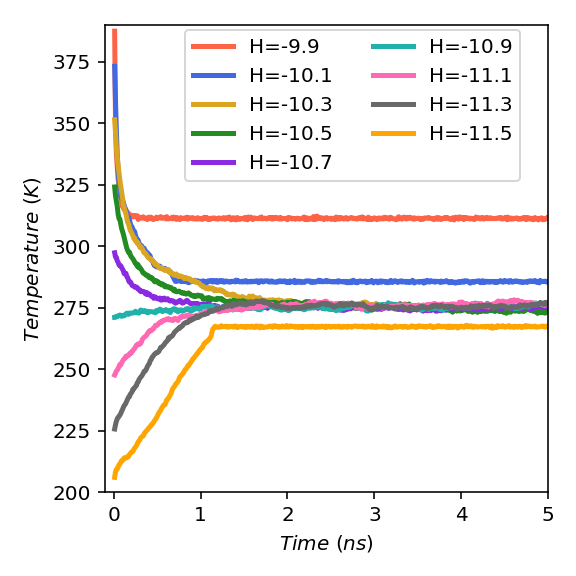
\includegraphics[width=0.5\textwidth]{PoteScan.png} 
\caption{The evolution of GNPT ensembles at distinct energy levels: Starting with a ice Ih/water coexisting state. Only the former 5ns equilibrium is plotted.
\label{fig:evolution} }
\end{figure}
Fig.\ref{fig:PTtemp-mw}
\begin{figure}[ht]
\centering{}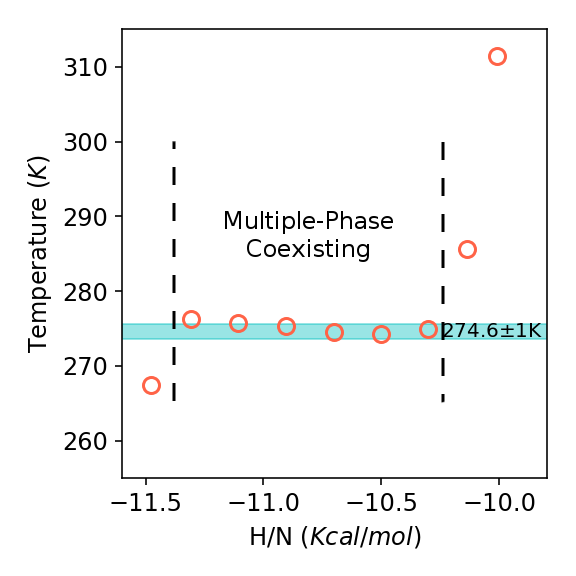
\includegraphics[width=0.5\textwidth]{PTtemp-mw.png} 
\caption{The phase transition temperature in GNPT ensembles. Dash line refers to 274.6K, the melting point for mW water proposed in previous study \cite{Molinero2009} . 
\label{fig:PTtemp-mw}} 
\end{figure}
Fig.\ref{fig:sizeeffect}

\begin{figure}[ht]
\centering{}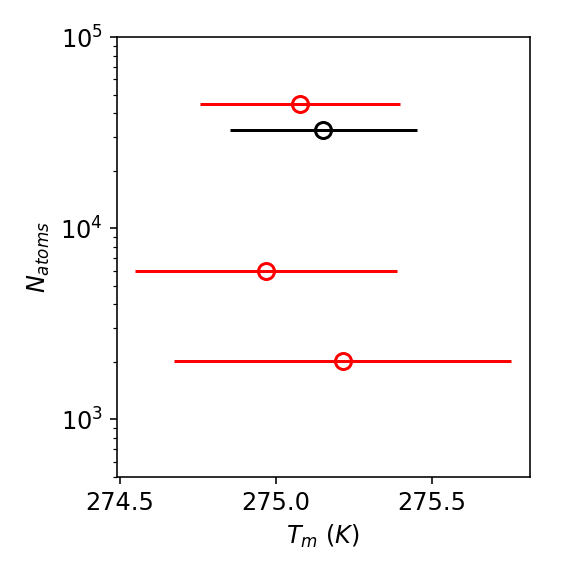
\includegraphics[width=0.5\textwidth]{size_effect.png} 
\caption{Size effect in GCE/GNPT method determined phase transition temperature. Data from Fig.\ref{fig:PTtemp-mw} is plot in black, the other data is extract from GNPT of 44800, 5971, 2030 water molecules, with size approximately 151 Å × 156 Å × 58 Å, 54 Å × 58 Å × 58 Å, 52Å × 56 Å × 22 Å,respectively.
\label{fig:sizeeffect}} 
\end{figure}
 This strategy is applied in full atom systems as well, the result is shown as below:
 
 

%\section{Conclusions} 
As summary, we show that the matching between the structure of interfacial water (IW) and the ice, involving both the ice-like oxygen lattice order and the hydrogen direction disorder, corresponds to the capability of substrates on the heterogeneous ice nucleation, only the lattice matching of substrates with ice may be not sufficient to aid ice nucleation. The result is helpful to finding and designing anti-/aid- freezing materials for application. 
    
%\section{Acknowledgement} 
The work is under the financial support of the NSFC Grant with No. 11574310, 11674345. C.-L. Wang thanks the support of the Youth Innovation Promotion Association, CAS. 

\section{Supplementary}

\begin{figure}[ht]
\centering{}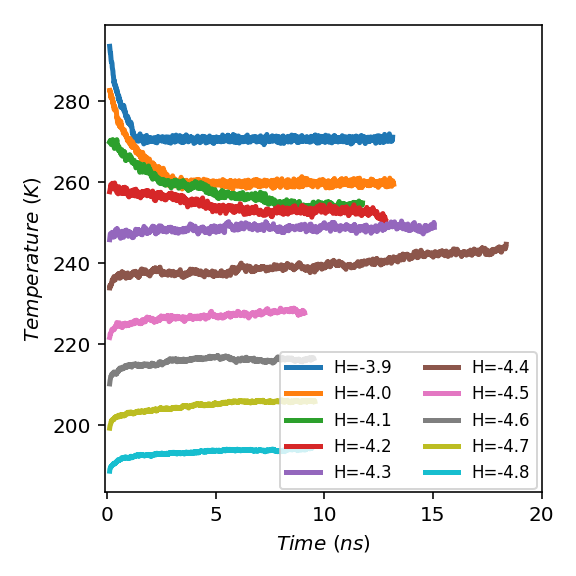
\includegraphics[width=0.5\textwidth]{PoteScan-2005.png} 
\caption{evolution of GNPT with tip4p-2005 water model
\label{fig:evolution-2005}} 
\end{figure}
\begin{figure}[ht]
\centering{}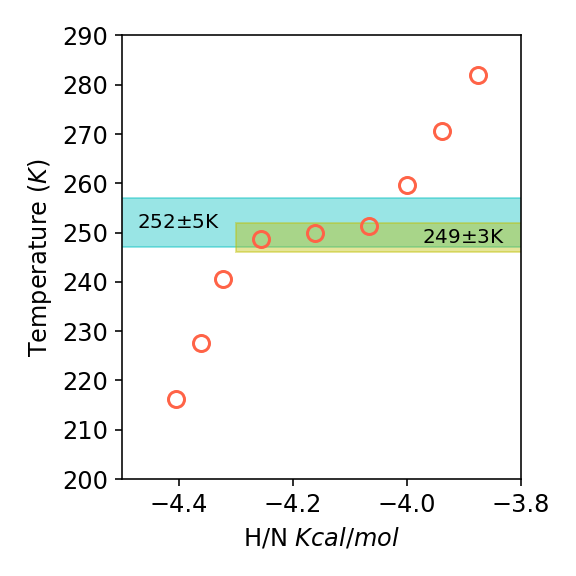
\includegraphics[width=0.5\textwidth]{PTtemp-2005.png} 
\caption{Phase transition temperature of GNPT with tip4p-2005 water model.
\label{fig:PTtemp-2005}} 
\end{figure}

\begin{figure}[ht]
\centering{}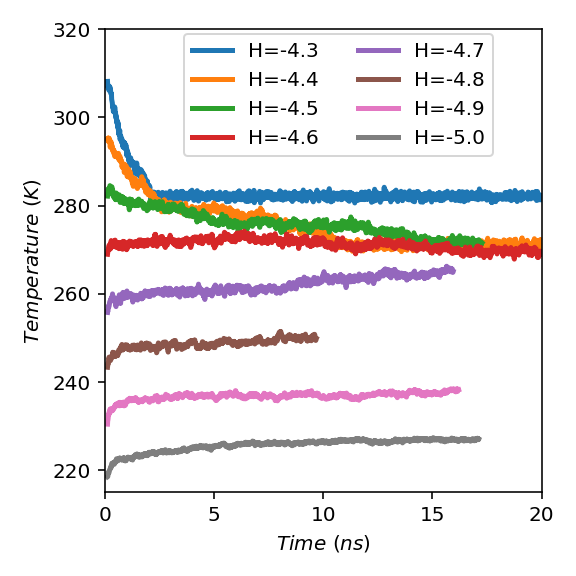
\includegraphics[width=0.5\textwidth]{PoteScan-ice.png} 
\caption{evolution of GNPT with tip4p-ice water model
\label{fig:evolution-ice}} 
\end{figure}
\begin{figure}[ht]
\centering{}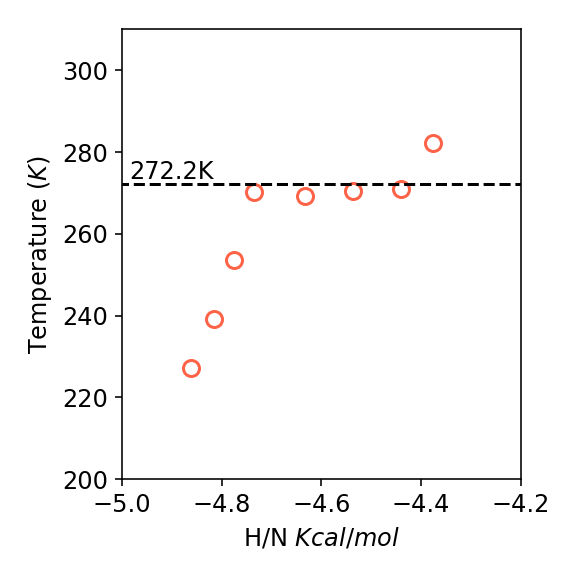
\includegraphics[width=0.5\textwidth]{PTtemp-ice.png} 
\caption{Phase transition temperature of GNPT with tip4p-icewater model.
\label{fig:PTtemp-ice}} 
\end{figure}




\begin{table}
\caption{Parameters of water model.}
\centering{}%
\begin{tabular}{cccccccc}
%\toprule 
\hline
{Model} & {$d_{oh}(\overset{\circ}{A})$} & { H-O-H}  & {$\sigma (\overset{\circ}{A})$}  & {$\epsilon/k (K)$} & {$q_H(e)$} & {  $T_m (K)$} 
\tabularnewline
%\midrule
\hline

{ TIP4P-2005} & { 0.9572} & {104.52}  & {3.3589}  & {93.20} & {0.5564} & {252.1} \tabularnewline
{ TIP4P-ICE} & { 0.9572} & {104.52}  & {3.1668}  & {106.1} & {0.5897} & {272.2} \tabularnewline
	{ mW} & { -} & {-}  & {-}  & {-} & {-} & {274.6}  \tabularnewline
%\bottomrule
\hline
\end{tabular}
\label{table:water model}
\end{table}

%%%END OF MAIN TEXT%%%

\bibliography{gce-PTtemp}
%You need to replace "rsc" on this line with the name of your .bib file
%\bibliographystyle{rsc} %the RSC's .bst file

\end{document}